%On the upper giant branch, near the location of the red giant branch bump, there is an observed episode of mixing whose efficiency is observed to depend on the initial mass and metallicity of the star \citep[e.g.][]{Gratton2000}. This has been assumed to related to thermohaline mixing (see citecite) but this has been disputed for both theoretical (citecite) and observational reasons \citep{TayarJoyce2022} (citecite). 
%\begin{minipage}{1.0\textwidth}
\begin{table*}[tb]
\begin{center}
\caption{Observed extra mixing drops in bins of mass and metallicity, corrected for the  0.1456 dex of unmixing observed that we assume is due to systematic errors. We also include  the reduced density ratios  calculated for each of these bins using the variety of models discussed in Section \ref{sec:mesa_results} \red{times 1000 for easier readability. We also report the number of stars in the pre-mixing and post-mixing phase for each bin.}}
\begin{tabular}{rrrrrrrr}
\hline
\multicolumn{1}{l}{M} & \multicolumn{1}{l}{[Fe/H]} & \multicolumn{1}{l} {$\Delta$[C/N]$_{\rm APK, cor}$} & {$\Delta$[C/N]$_{\rm Shet, cor}$}  & \multicolumn{1}{l}{$r_{\rm Brown, 1}$} & \multicolumn{1}{l}{$r_{\rm Kip, 1}$} & \multicolumn{1}{l}{$r_{\rm Kip, 2}$} & \multicolumn{1}{l}{$r_{\rm Kip, 700}$} \\ \hline \hline
0.9 & -1.2 & \multicolumn{1}{l}{} & \multicolumn{1}{r}{0.67} & 0.00006 & 0.00013 & 0.00006 & 0.00013 \\ 
0.9 & -1 & \multicolumn{1}{l}{} & \multicolumn{1}{r}{0.48} & 0.00008 & 0.00015 & 0.00008 & 0.00017 \\ 
0.9 & -0.8 & 0.52 & \multicolumn{1}{r}{0.36} & 0.00010 & 0.00016 & 0.00009 & 0.00022 \\ 
0.9 & -0.6 & 0.29 & \multicolumn{1}{r}{0.27} & 0.00012 & 0.00018 & 0.00012 & 0.0003 \\ 
0.9 & -0.4 & 0.16 & \multicolumn{1}{r}{0.21} & 0.00015 & 0.0002 & 0.00015 & 0.00038 \\ 
1.1 & -0.4 & 0.13 &  & 0.00020 & 0.00024 & 0.00020 & 0.00031 \\ 
1.3 & -0.4 & 0.07 &  & 0.00029 & 0.00027 & 0.00037 & 0.00029 \\ 
1.5 & -0.4 & 0.10 &  & 0.00044 & 0.00029 & 0.00051 & 0.00029 \\ 
0.9 & -0.2 & 0.20 &  & 0.00020 & 0.00023 & 0.00019 & 0.00053 \\ 
1.1 & -0.2 & 0.11 &  & 0.00027 & 0.00028 & 0.00026 & 0.00043 \\ 
1.3 & -0.2 & 0.09 &  & 0.00037 & 0.00032 & 0.00044 & 0.0004 \\ 
1.5 & -0.2 & 0.10 &  & 0.00055 & 0.00034 & 0.00062 & 0.0004 \\ 
1.1 & 0 & 0.14 &  & 0.00034 & 0.00032 & 0.00033 & 0.00055 \\ 
1.3 & 0 & 0.05 &  & 0.00047 & 0.00037 & 0.00054 & 0.00053 \\ 
1.5 & 0 & 0.09 &  & 0.00068 & 0.0004 & 0.00076 & 0.00053 \\ 
1.7 & 0 & 0.02 &  & 0.00100 & 0.00042 & 0.00093 & 0.00057 \\ 
1.1 & 0.2 & 0.12 &  & 0.00044 & 0.00038 & 0.00043 & 0.00072 \\ 
1.3 & 0.2 & 0.00 &  & 0.00062 & 0.00044 & 0.00068 & 0.0007 \\ 
1.5 & 0.2 & 0.01 &  & 0.00091 & 0.00047 & 0.00098 & 0.00074 \\ 
1.7 & 0.2 & 0.00 &  & 0.00136 & 0.00051 & 0.00119 & 0.00082 \\ 
1.1 & 0.4 & 0.04 &  & 0.00059 & 0.00045 & 0.00058 & 0.00093 \\ 
1.3 & 0.4 & 0.01 &  & 0.00086 & 0.00052 & 0.00092 & 0.00094 \\ \hline
\end{tabular}
\label{tab:obsdata}
\end{center}
\end{table*}
%\end{minipage}

Recently, modern spectroscopic surveys have begun collecting measurements of mixing diagnostics for large samples of stars whose masses are also well constrained, making it possible to compare %the observed trends of mixing 
\textbf{observed mixing trends}
to the predictions of the 
%variety of 
theoretical models discussed above (Section \ref{sec:parameterizations}) by using one dimensional stellar evolution models to estimate the relevant fluid parameters of these stars given their masses and metallicities (Section \ref{sec:mesa_results}). 
%
We choose for this work to use the carbon-to-nitrogen ratios, \textbf{[C/N],} measured from the Apache Point Galactic Evolution Experiment \citep[APOGEE, ][]{Majewski2015,Majewski2017}. APOGEE is a Sloan Digital Sky Survey III and IV \citep{Blanton2017} project using the 2.5 meter Sloan Telescope \citep{Gunn2006} and the APOGEE spectrograph \citep{Wilson2019} to obtain medium resolution (R $\sim$ 22,500) spectra of large numbers of stars across the galaxy \citep{Zasowski2017, Beaton2021,Santana2021}. These spectra are homogeneously reduced and analyzed using the ASPCAP pipeline \citep{Nidever2015, Zamora2015, GarciaPerez2016} and the resulting stellar parameters are then calibrated using asteroseismic, cluster, and field data \citep{Holtzman2015,Holtzman2018, Jonsson2020}. We choose to use the APOGEE data because this calibration work has already been done and asteroseismology has been used to estimate stellar masses \textbf{in a way that has been translated across the survey, [What does this mean? - MJ]}, though \sout{we acknowledge that} similar work could likely be done with, for example, the lithium abundances measured by the GALAH survey \citep{buder2019} or the \ctwelvecthirteen data estimated from the APOGEE data using the Brussels Automatic Code
for Characterizing High accUracy Spectra \citep[BACCHUS,][]{Masseron2016_BACCHUS} pipeline (C. Hayes, submitted). 

We also note that the evolution of [C/N] is in some ways simpler for these low mass stars than other mixing diagnostics. Unlike lithium, its abundance at the surface does not change significantly during the main sequence due to the effects of rotational and other mixing processes \citep{Iben1967}. Its initial ratio seems to be somewhat metallicity dependent \citep{Shetrone2019}%, JackandMarcifSubmitted}
, with higher values at lower metallicity. As stars reach the first dredge up, there is a strong, rapid, mass dependent change in the surface [C/N] ratio \citep{MasseronGilmore2015, Martig2016, Ness2016, Spoo2022}. The [C/N] ratio at the surface then remains constant until stars reach the red giant branch bump, after which there seems to be another rapid drop in the [C/N] ratio, particularly in stars of low metallicity; it is this drop that has been associated with thermohaline mixing. On the upper giant branch for stars of particularly low metallicities, there are some suggestions of Upper RGB extra mixing \citep{Shetrone2019} which is not well motivated theoretically, but it is separate from the processes we are discussing here.

To estimate the amount of extra mixing in these stars near the bump, which thermohaline models suggest should trace the %compositional Nusselt number (\Numu) and 
mixing rates $\Dth$ described above, %we follow the work of 
\citet{Shetrone2019} estimated the drop in [C/N] just above the red giant branch bump. That work used $\alpha$-element enhanced, and therefore old and low-mass ($\sim$0.9 \msun), first ascent red giant branch stars and binned them in bins of 0.2 dex in metallicity. The location of the red giant branch bump was identified empirically as an overdensity of stars at a particular surface gravity in each bin. They then identified the region of gravities around the first dredge up and the red giant branch bump, in each of these regions they fit a hyperbolic tangent function to measure the location and size of the drops in the [C/N] ratio. For simplicity, we have reproduced their results in Table \ref{tab:obsdata}. 

We add to their analysis a sample of higher metallicity stars with asteroseismic masses from the APOGEE-Kepler overlap sample \citep[APOKASC,][]{Pinsonneault2014, Pinsonneault2018}. We do this because, according to our analysis in Section \ref{sec:mesa_results}, higher mass, higher metallicity stars probe larger values of the reduced density ratio, $r$. Specifically, we first bin the stars in mass (0.2 \msun), metallicity (0.2 dex). For consistency with \citet{Pinsonneault2018} and \citet{Shetrone2019}, we use the Data Release 14 \citet{DR14} abundances, although we note that while the scale seems to shift between releases, the rank ordering does not change very much \citep{Spoo2022} which means that the conclusions of this analysis are not strongly affected by the choice of Data Release or seismic parameters.

Unlike the \citet{Shetrone2019} analysis, there are not sufficient stars near the bump in each bin to detect and measure the extra mixing directly as it happens in the asteroseismic sample. Instead, we define a `pre-mixing' bin of stars between \logg\ of  3.4 and 2.8 dex whose oscillations have identified them as first ascent red giants \citep{Elsworth2019}, as well as a `post-mixing' bin of RGB stars with surface gravities between 2.3 and 1.0 dex. We then compute the average [C/N] of stars in each of the pre-mixing and post-mixing bins. If both bins had at least three stars, then the difference is plotted in Figure \ref{fig:obssquare}. Because of the calibration and choices in the analysis pipeline
%We then identify the range of surface gravities that represent stars around the red giant branch bump, adopting 1.5 $<$ \logg $<$ 2.9 dex for consistency with \citet{Shetrone2019}. Finally, we fit a hyperbolic tangent function to the [C/N] ratio as a function of surface gravity, reporting the midpoint of the transition, and the total change in [C/N] in Table \ref{tab:obs}.
%For this analysis, we use the most recent Data Release 17 \citep{DR17} measurements of carbon and nitrogen, combined with the most recent astroseismic results (M. Pinsonneault et al. 2022, in prep). Because of the challenges of calibration, as well as the changes to the analysis pipelines between data releases 
\citep[see e.g.][]{Holtzman2018,Jonsson2020, vsmith_apogee_dr16_2021}, the scale of the abundances% actual abundances
, particularly for carbon and nitrogen,
are somewhat uncertain.
%often change between data releases. While the rank ordering of stars of a particular surface gravity tends to be robust \citep{Martig2016,Ness2016}, 
There are sometimes small trends with surface gravity and temperature that are not fully removed in the calibration process. This is notable in our measurement results here, in the highest mass, highest metallicity bins, we formally measure `unmixing' near the red giant branch bump, which is inconsistent both with theoretical expectations and with measurements from other sources. Following discussions with the APOGEE team (C. Hayes, private communication), we have decided to correct for these effects by correcting the bin with the most `unmixing' to have 0 mixing, and subtracting that change from all of the other bins under the assumption that the systematic measurement errors are consistent for stars of similar temperatures and gravities. Because we are most interested here in the trend in mixing amounts as a function of the stellar parameters, we don't expect this shift to alter the results of this analysis, but we emphasize that care should be taken by future users of this data. 

%\textbf{ if we end up having a bunch of authors on this, we should add Chris Hayes. }
%FIGURE omgcomp---------------------------------------------------
\begin{figure}[!tb]
\begin{center}
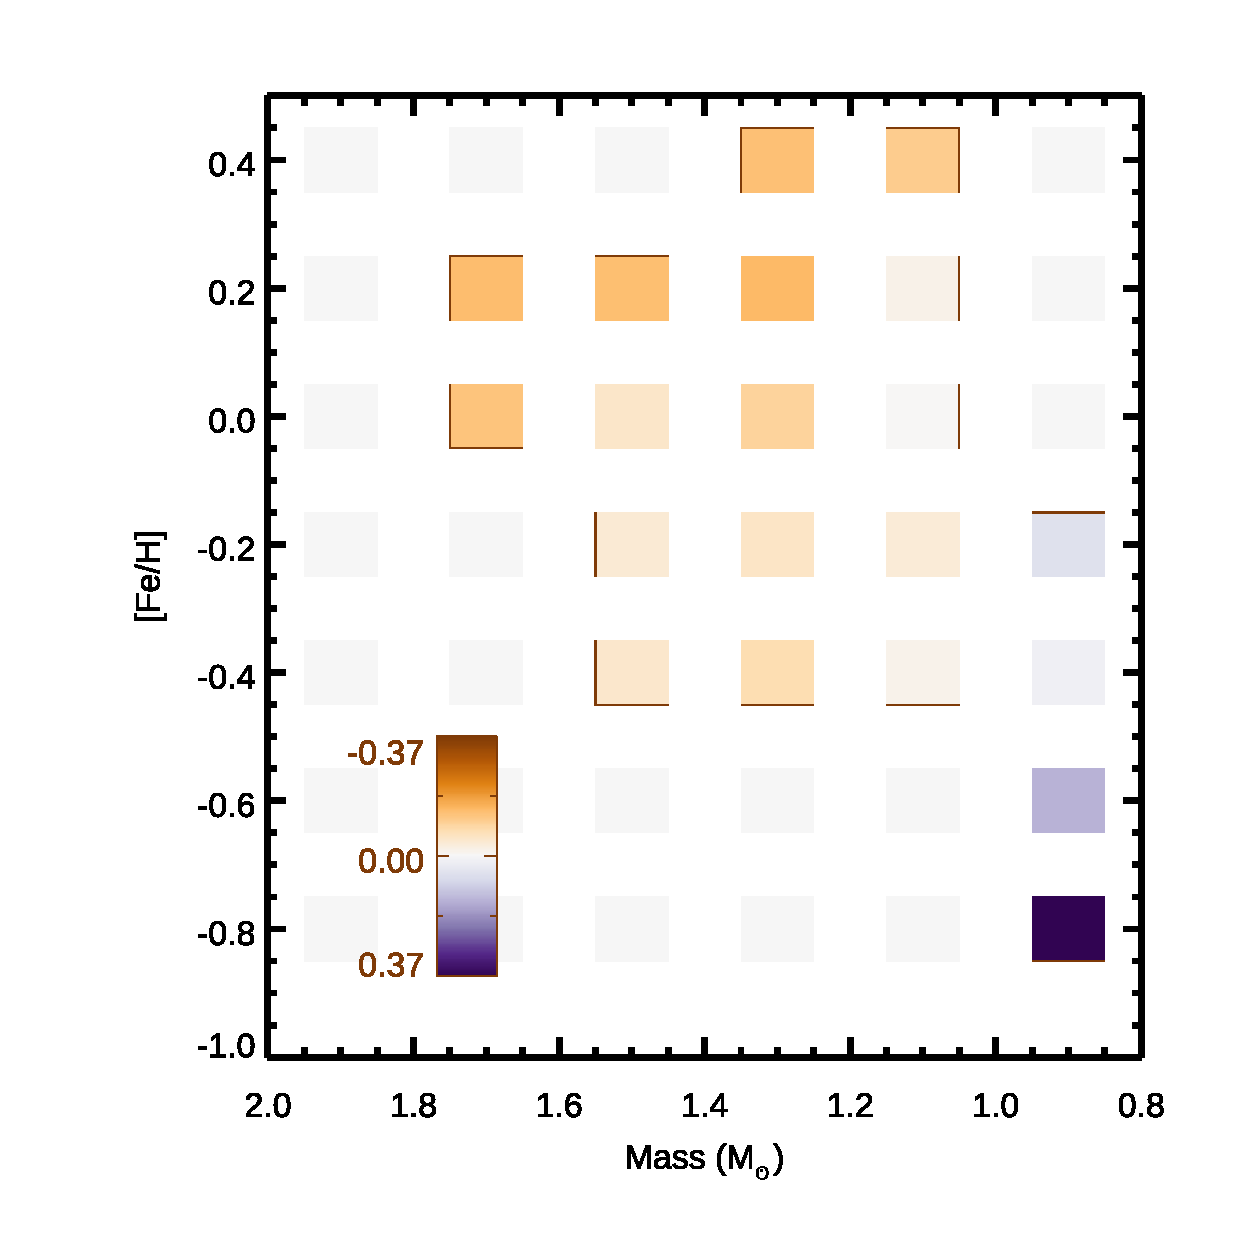
\includegraphics[width=9cm,clip=true, trim=0.5in 0in 0in 0in]{./figures/Mfeh5c_mixingCRGBdr14v6.eps}%[width=9cm, clip=true, trim=1in 1in 1in 1in]{./Figs/omgcomp.eps}
\caption{The difference in average [C/N] (box color) between stars significantly below the RGB bump and those significantly above the bump, as a function of stellar mass and metallicity. The gradient is consistent with previous work, with lower mass, lower metallicity stars having more extra mixing (purple), but there is clearly an unphysical `unmixing' trend (orange) that needs to be removed (see text). We highlight only bins with a sufficient number of stars both below and above the bump.}
%There seems to be some moderate evidence of core-envelope recoupling as the stars evolve on the secondary clump, although more measurements of evolved stars with slowly rotating surfaces would strengthen this conclusion.} %\textbf{mark a line for the selection effect?} }
\label{fig:obssquare}
\end{center}
\end{figure}
%FIGURE omgcomp---------------------------------------------------

%if we use shetrone straight and then dr17, they wont be on the same scale. deeply annoying. could correct, or redo the shetrone analysis. 
%also need to decide what apokasc we use (2 is public, 3 is still in limbo as far as i can tell. 2 is technically dr16, but i can cross with the dr17 c/n. JT need to check how much this matters)




%Using the observed data from DR16 APOKASC (or cite Shetrone 2019 if that's enough) describe pre-bump ID, bump ID, post bump range. 

%make same plot of mass versus metallicity, color code by amount of mixing (delta [C/N] ) 

